\section{Bewertung der Ergebnisse hinsichtlich der Zielvorgabe}

Nachfolgend soll nun die Ergebnisse der Migration bezüglich der Erfüllung der in Kapitel~\ref{chap:analysis} definierten Ziele untersucht werden. Die erste Zielsetzung war hierbei die Erkennung weiterer Typ- und Programmfehler.

\subsection{Erkennung weiterer Typ- und Programmfehler}
\label{goal:new-type-errors}


% Der TypeScript-Compiler besitzt wie in Abschnitt~\ref{sec:typescript} beschrieben verschiedene Optionen, um die Striktheit der Typüberprüfungen zu erhöhen. Diese kann durch Setzen der Option \enquote{\code{strict}} angepasst werden, sodass daraufhin deutlich mehr Ausdrücke als Typfehler betrachtet werden.

% TODO: histogramme mit top 8 fehlern oder so strikt vs nicht-strikt
% TODO: erklärung: wo kommen diese fehler her? welche davon sind tatsächlich problematisch? welche nur bs von ts?
% TODO: ein paar beispiele für echte probleme

\subsection{Unterstützung externer Bibliotheken}

% TODO: vergleich flow-typed definitely typed
% TODO: 3 "schöne" bibs rauspicken (react, redux, lodash, datefns?) und libdefs vergleichen

\subsection{Performance der Typüberprüfungen}

\subsubsection{Laufzeitmessung vollständiger Typüberprüfungen}

Eine weitere Zielsetzung des Wechsels zu TypeScript war die Performance der Typüberprüfungen zu steigern bzw. diese zumindest nicht zu verschlechtern. Nachdem die Migration der zwei Projekte abgeschlossen war, konnten die Laufzeiten der vollständigen Typüberprüfung durch Flow bzw. TypeScript ermittelt werden. Die Messung der Zeitdauer von inkrementellen Überprüfungen durch den Flow- bzw. TypeScript-Sprachserver konnte nicht unabhängig von der Ausführung eines Editors  durchgeführt werden, sodass dieser Aspekt nachfolgend nicht betrachtet werden kann, da die Gefahr besteht, dass der Editor die Ergebnisse verfälscht.

Zur Bestimmung der Laufzeiten wurden für Flow und TypeScript jeweils 100 Proben (\textit{Samples}) mithilfe des GNU-Programms \textit{time}~\autocite{GNU_TIME} gemessen und die zehn kleinsten und größten Werte daraufhin verworfen, um den Einfluss von \enquote{Ausreißern} zu minimieren. Aus den verbleibenden 80 Werten wurde anschließend der Mittelwert gebildet und die Standardabweichung berechnet. Dabei wurde in allen Messungen die zum damaligen Zeitpunkt aktuelle Version~3.5 von TypeScript und die von TeamShirts eingesetzte Version~0.96 von Flow verwendet. Um auch den Einfluss von unterschiedlich leistungsfähiger Hardware miteinzubeziehen, wurden die Messreihen auf vier verschiedenen Systemen durchgeführt:

\begin{enumerate}[label=\Alph*.]
  \item AMD Phenom II X6 1055T Prozessor mit 2,9~GHz\footnote{Es wird jeweils der Grundtakt des Prozessors und nicht der maximal mögliche Wert durch dynamische Übertaktung angegeben.} und 6\footnote{} Rechenkernen (2010)\\16~GB Arbeitsspeicher, Solid State Drive, Arch Linux
  \item Intel Core i5-4258U Prozessor mit 2,4~GHz und 4 Rechenkernen (2013)\\8~GB Arbeitsspeicher, Solid State Drive, Arch Linux
  \item Intel Core i5-4210M Prozessor mit 2,6~GHz und 4 Rechenkernen (2014)\\16~GB Arbeitsspeicher, Solid State Drive, Arch Linux
  \item Intel Core i7-6700 Prozessor mit 3,4~GHz und 8 Rechenkernen (2015)\\32~GB Arbeitsspeicher, Solid State Drive, Debian Linux
\end{enumerate}

Die durch diese Methodik ermittelten Messwerte, deren Standardabweichung und die relative Veränderung der Laufzeiten werden in Tabelle~\ref{tab:performance-complete} für beide Projekte aufgelistet: Offensichtlich beschleunigen modernere, performante Prozessoren mit höherer Taktfrequenz und größeren Caches generell die Typüberprüfung durch Flow bzw. TypeScript. Die These, dass TypeScript schneller als Flow sei, lässt sich aber nur anhand des Projekts Helios für die Systeme B, C und D belegen (vgl. negative Werte für relative Veränderung der Laufzeit). Bei Components ist TypeScript dagegen stets deutlich langsamer als Flow.

\medbreak
\begingroup
\setlength{\tabcolsep}{7pt}
\begin{table}[tbh]
  \small
  \begin{tabu} to \textwidth {@{}rrrrrr|rrrrrX@{}}
    \midrule
    {} & \multicolumn{2}{l}{\libertineSB{Flow}} & \multicolumn{2}{l}{\libertineSB{TypeScript}} & {} & \multicolumn{2}{l}{\libertineSB{Flow}} & \multicolumn{2}{l}{\libertineSB{TypeScript}} & {}\\
    \rowfont[c]{} \libertineSB{S} & Laufzeit & s & Laufzeit & s & rel. $\Delta$ & Laufzeit & s & Laufzeit & s & rel. $\Delta$ & {}\\
    \midrule
    A & 7,87 & 0,09 & 15,50 & 0,08 & 97,0\% & 12,20 & 0,16 & 13,06 & 0,70 &   7,1\% & {} \\
    B & 6,86 & 0,05 & 10,59 & 0,06 & 54,4\% & 10,90 & 0,33 &  8,49 & 0,16 & -22,1\% & {} \\
    C & 6,50 & 0,02 &  9,56 & 0,05 & 47,1\% & 11,70 & 0,07 &  7,63 & 0,04 & -34,8\% & {} \\
    D & 3,38 & 0,02 &  6,41 & 0,04 & 89,6\% &  5,15 & 0,02 &  4,94 & 0,03 &  -4,1\% & {} \\
    \midrule
    {} & \multicolumn{5}{c}{\large\textsc{components}} & \multicolumn{5}{c}{\large\textsc{helios}} & {}\\
    \midrule
  \end{tabu}
  \caption{Durchschnittliche Laufzeit in Sekunden, Standardabweichung (s) und relative Veränderung der Zeitspanne (rel. $\Delta$) der vollständigen Typüberprüfung der Projekte Components und Helios durch Flow 0.96 und TypeScript 3.5 auf verschiedenen Hardware-Systemen (S).}
  \label{tab:performance-complete}
\end{table}
\endgroup


Wie im Grundlagenteil bereits ausgeführt wird die Berechnung der Typkorrektheit durch Flow stark parallelisiert, um diese zu verschnellern. TypeScript bietet keine Unterstützung für eine nebenläufige Typüberprüfung durch mehrere Threads~\autocite{TS:NO_MULTICORE}, sodass die Performance hier vorrangig von der Leistungsfähigkeit der einzelnen Prozessorkerne abzuhängen scheint. Diese These wird durch die gemessenen Daten unterstützt, denn je performanter die Prozessoren sind, desto kleiner kleiner wird die Differenz zwischen den Laufzeiten von Flow und TypeScript bei Components bzw. desto größer wird diese bei Helios.
Für System D scheint jedoch die Parallelisierung von Flow aufgrund der hohen Zahl von acht Rechenkernen den größeren Effekt zu haben, als die Leistungsfähigkeit der einzelnen Kerne. Weil die Systeme B und C jeweils nur über vier Prozessorkerne verfügen, ist der Einfluss der Nebenläufigkeit hier kleiner. Als einen möglichen Grund warum Components im Vergleich zu Helios durch Flow insgesamt schneller überprüft werden kann, kann angeführt werden, dass dieses Projekt aus einer Vielzahl unabhängiger Komponenten besteht deren Verarbeitung somit gut durch Flow parallelisiert werden kann. In Helios besteht eine größere Abhängigkeit der Module zueinander.

\subsubsection{Einfluss von Parallelisierung auf die Laufzeiten}

Der Einfluss der Parallelisierung auf die Laufzeit der Berechnungen soll im Folgenden näher untersucht werden. Hierfür wurde eine weitere Testreihe durchgeführt in welcher die Zahl der einsetzbaren Rechenkerne für die Berechnung durch das Linux-Programm \textit{taskset}~\autocite{TASKSET} eingeschränkt wird. Dabei wird dem Prozess durch den Scheduler des Betriebssystems zunächst lediglich ein Rechenkern, dann zwei usw. zugeordnet. Abbildung~\ref{fig:plot-cores} auf Seite~\pageref{fig:plot-cores} zeigt jeweils ein Diagramm für Components und Helios, welche die Beeinflussung des Laufzeitverhaltens durch diese Einschränkung grafisch darstellen. Die exakten Messwerte und deren Standardabweichung wird darüber hinaus in Tabelle~\ref{tab:performance-cores} aufgelistet.

Sowohl bei Flow, als auch bei TypeScript ermöglicht bereits die Verwendung von zwei Rechenkernen eine starke Verbesserung der Laufzeiten im Vergleich zu einem einzigen Kern. Obwohl TypeScript eine Kompilierung durch mehrere Prozessorkerne grundsätzlich nicht unterstützt, wird auch dieser Prozess so beschleunigt, weil der TypeScript Compiler durch Node.js ausgeführt wird und diese Umgebung mehrere Threads startet, um beispielsweise teure Ein- und Ausgabeoperationen auf weitere Rechenkerne auszulagern~\autocite{NODE:THREADS}. Für mehr als drei Kerne bleibt die Laufzeit von TypeScript daraufhin in etwa konstant. Die Laufzeit von Flow verringert sich hingegen mit zunehmender Zahl zur Verfügung stehender Rechenkerne aufgrund der Multithreading-Unterstützung stetig. Ab etwa fünf Kernen sind die Zugewinne allerdings nur noch gering, was auf den zunehmend größeren Overhead durch die notwendige Synchronisierung der Threads zurückgeführt werden könnte.

\begin{figure}[tbp]
  \centering

  % GNUPLOT: LaTeX picture with Postscript
\begingroup
  \makeatletter
  \providecommand\color[2][]{%
    \GenericError{(gnuplot) \space\space\space\@spaces}{%
      Package color not loaded in conjunction with
      terminal option `colourtext'%
    }{See the gnuplot documentation for explanation.%
    }{Either use 'blacktext' in gnuplot or load the package
      color.sty in LaTeX.}%
    \renewcommand\color[2][]{}%
  }%
  \providecommand\includegraphics[2][]{%
    \GenericError{(gnuplot) \space\space\space\@spaces}{%
      Package graphicx or graphics not loaded%
    }{See the gnuplot documentation for explanation.%
    }{The gnuplot epslatex terminal needs graphicx.sty or graphics.sty.}%
    \renewcommand\includegraphics[2][]{}%
  }%
  \providecommand\rotatebox[2]{#2}%
  \@ifundefined{ifGPcolor}{%
    \newif\ifGPcolor
    \GPcolortrue
  }{}%
  \@ifundefined{ifGPblacktext}{%
    \newif\ifGPblacktext
    \GPblacktexttrue
  }{}%
  % define a \g@addto@macro without @ in the name:
  \let\gplgaddtomacro\g@addto@macro
  % define empty templates for all commands taking text:
  \gdef\gplbacktext{}%
  \gdef\gplfronttext{}%
  \makeatother
  \ifGPblacktext
    % no textcolor at all
    \def\colorrgb#1{}%
    \def\colorgray#1{}%
  \else
    % gray or color?
    \ifGPcolor
      \def\colorrgb#1{\color[rgb]{#1}}%
      \def\colorgray#1{\color[gray]{#1}}%
      \expandafter\def\csname LTw\endcsname{\color{white}}%
      \expandafter\def\csname LTb\endcsname{\color{black}}%
      \expandafter\def\csname LTa\endcsname{\color{black}}%
      \expandafter\def\csname LT0\endcsname{\color[rgb]{1,0,0}}%
      \expandafter\def\csname LT1\endcsname{\color[rgb]{0,1,0}}%
      \expandafter\def\csname LT2\endcsname{\color[rgb]{0,0,1}}%
      \expandafter\def\csname LT3\endcsname{\color[rgb]{1,0,1}}%
      \expandafter\def\csname LT4\endcsname{\color[rgb]{0,1,1}}%
      \expandafter\def\csname LT5\endcsname{\color[rgb]{1,1,0}}%
      \expandafter\def\csname LT6\endcsname{\color[rgb]{0,0,0}}%
      \expandafter\def\csname LT7\endcsname{\color[rgb]{1,0.3,0}}%
      \expandafter\def\csname LT8\endcsname{\color[rgb]{0.5,0.5,0.5}}%
    \else
      % gray
      \def\colorrgb#1{\color{black}}%
      \def\colorgray#1{\color[gray]{#1}}%
      \expandafter\def\csname LTw\endcsname{\color{white}}%
      \expandafter\def\csname LTb\endcsname{\color{black}}%
      \expandafter\def\csname LTa\endcsname{\color{black}}%
      \expandafter\def\csname LT0\endcsname{\color{black}}%
      \expandafter\def\csname LT1\endcsname{\color{black}}%
      \expandafter\def\csname LT2\endcsname{\color{black}}%
      \expandafter\def\csname LT3\endcsname{\color{black}}%
      \expandafter\def\csname LT4\endcsname{\color{black}}%
      \expandafter\def\csname LT5\endcsname{\color{black}}%
      \expandafter\def\csname LT6\endcsname{\color{black}}%
      \expandafter\def\csname LT7\endcsname{\color{black}}%
      \expandafter\def\csname LT8\endcsname{\color{black}}%
    \fi
  \fi
    \setlength{\unitlength}{0.0500bp}%
    \ifx\gptboxheight\undefined%
      \newlength{\gptboxheight}%
      \newlength{\gptboxwidth}%
      \newsavebox{\gptboxtext}%
    \fi%
    \setlength{\fboxrule}{0.5pt}%
    \setlength{\fboxsep}{1pt}%
\begin{picture}(7360.00,4520.00)%
    \gplgaddtomacro\gplbacktext{%
      \csname LTb\endcsname%%
      \put(596,652){\makebox(0,0)[r]{\strut{}$3$}}%
      \csname LTb\endcsname%%
      \put(596,1107){\makebox(0,0)[r]{\strut{}$4$}}%
      \csname LTb\endcsname%%
      \put(596,1563){\makebox(0,0)[r]{\strut{}$5$}}%
      \csname LTb\endcsname%%
      \put(596,2018){\makebox(0,0)[r]{\strut{}$6$}}%
      \csname LTb\endcsname%%
      \put(596,2474){\makebox(0,0)[r]{\strut{}$7$}}%
      \csname LTb\endcsname%%
      \put(596,2929){\makebox(0,0)[r]{\strut{}$8$}}%
      \csname LTb\endcsname%%
      \put(596,3384){\makebox(0,0)[r]{\strut{}$9$}}%
      \csname LTb\endcsname%%
      \put(596,3840){\makebox(0,0)[r]{\strut{}$10$}}%
      \csname LTb\endcsname%%
      \put(596,4295){\makebox(0,0)[r]{\strut{}$11$}}%
      \csname LTb\endcsname%%
      \put(1410,448){\makebox(0,0){\strut{}1}}%
      \csname LTb\endcsname%%
      \put(2111,448){\makebox(0,0){\strut{}2}}%
      \csname LTb\endcsname%%
      \put(2813,448){\makebox(0,0){\strut{}3}}%
      \csname LTb\endcsname%%
      \put(3515,448){\makebox(0,0){\strut{}4}}%
      \csname LTb\endcsname%%
      \put(4216,448){\makebox(0,0){\strut{}5}}%
      \csname LTb\endcsname%%
      \put(4918,448){\makebox(0,0){\strut{}6}}%
      \csname LTb\endcsname%%
      \put(5620,448){\makebox(0,0){\strut{}7}}%
      \csname LTb\endcsname%%
      \put(6321,448){\makebox(0,0){\strut{}8}}%
    }%
    \gplgaddtomacro\gplfronttext{%
      \csname LTb\endcsname%%
      \put(158,2473){\rotatebox{-270}{\makebox(0,0){\strut{}\small durchschnittliche Laufzeit in s}}}%
      \csname LTb\endcsname%%
      \put(3865,142){\makebox(0,0){\strut{}\small Anzahl eingesetzter Prozessorkerne}}%
      \csname LTb\endcsname%%
      \put(3865,3989){\makebox(0,0){\strut{}\small\bfseries Components}}%
      \csname LTb\endcsname%%
      \put(6158,4010){\makebox(0,0)[r]{\strut{}\small Flow}}%
      \csname LTb\endcsname%%
      \put(6158,3806){\makebox(0,0)[r]{\strut{}\small TypeScript}}%
    }%
    \gplbacktext
    \put(0,0){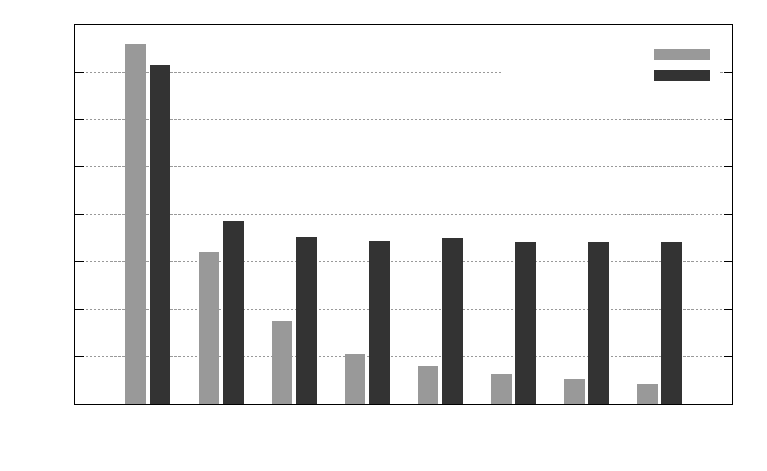
\includegraphics{../data/performance/plots/cores/components-plot}}%
    \gplfronttext
  \end{picture}%
\endgroup


  \vspace{.5\baselineskip}

  % GNUPLOT: LaTeX picture with Postscript
\begingroup
  \makeatletter
  \providecommand\color[2][]{%
    \GenericError{(gnuplot) \space\space\space\@spaces}{%
      Package color not loaded in conjunction with
      terminal option `colourtext'%
    }{See the gnuplot documentation for explanation.%
    }{Either use 'blacktext' in gnuplot or load the package
      color.sty in LaTeX.}%
    \renewcommand\color[2][]{}%
  }%
  \providecommand\includegraphics[2][]{%
    \GenericError{(gnuplot) \space\space\space\@spaces}{%
      Package graphicx or graphics not loaded%
    }{See the gnuplot documentation for explanation.%
    }{The gnuplot epslatex terminal needs graphicx.sty or graphics.sty.}%
    \renewcommand\includegraphics[2][]{}%
  }%
  \providecommand\rotatebox[2]{#2}%
  \@ifundefined{ifGPcolor}{%
    \newif\ifGPcolor
    \GPcolortrue
  }{}%
  \@ifundefined{ifGPblacktext}{%
    \newif\ifGPblacktext
    \GPblacktexttrue
  }{}%
  % define a \g@addto@macro without @ in the name:
  \let\gplgaddtomacro\g@addto@macro
  % define empty templates for all commands taking text:
  \gdef\gplbacktext{}%
  \gdef\gplfronttext{}%
  \makeatother
  \ifGPblacktext
    % no textcolor at all
    \def\colorrgb#1{}%
    \def\colorgray#1{}%
  \else
    % gray or color?
    \ifGPcolor
      \def\colorrgb#1{\color[rgb]{#1}}%
      \def\colorgray#1{\color[gray]{#1}}%
      \expandafter\def\csname LTw\endcsname{\color{white}}%
      \expandafter\def\csname LTb\endcsname{\color{black}}%
      \expandafter\def\csname LTa\endcsname{\color{black}}%
      \expandafter\def\csname LT0\endcsname{\color[rgb]{1,0,0}}%
      \expandafter\def\csname LT1\endcsname{\color[rgb]{0,1,0}}%
      \expandafter\def\csname LT2\endcsname{\color[rgb]{0,0,1}}%
      \expandafter\def\csname LT3\endcsname{\color[rgb]{1,0,1}}%
      \expandafter\def\csname LT4\endcsname{\color[rgb]{0,1,1}}%
      \expandafter\def\csname LT5\endcsname{\color[rgb]{1,1,0}}%
      \expandafter\def\csname LT6\endcsname{\color[rgb]{0,0,0}}%
      \expandafter\def\csname LT7\endcsname{\color[rgb]{1,0.3,0}}%
      \expandafter\def\csname LT8\endcsname{\color[rgb]{0.5,0.5,0.5}}%
    \else
      % gray
      \def\colorrgb#1{\color{black}}%
      \def\colorgray#1{\color[gray]{#1}}%
      \expandafter\def\csname LTw\endcsname{\color{white}}%
      \expandafter\def\csname LTb\endcsname{\color{black}}%
      \expandafter\def\csname LTa\endcsname{\color{black}}%
      \expandafter\def\csname LT0\endcsname{\color{black}}%
      \expandafter\def\csname LT1\endcsname{\color{black}}%
      \expandafter\def\csname LT2\endcsname{\color{black}}%
      \expandafter\def\csname LT3\endcsname{\color{black}}%
      \expandafter\def\csname LT4\endcsname{\color{black}}%
      \expandafter\def\csname LT5\endcsname{\color{black}}%
      \expandafter\def\csname LT6\endcsname{\color{black}}%
      \expandafter\def\csname LT7\endcsname{\color{black}}%
      \expandafter\def\csname LT8\endcsname{\color{black}}%
    \fi
  \fi
    \setlength{\unitlength}{0.0500bp}%
    \ifx\gptboxheight\undefined%
      \newlength{\gptboxheight}%
      \newlength{\gptboxwidth}%
      \newsavebox{\gptboxtext}%
    \fi%
    \setlength{\fboxrule}{0.5pt}%
    \setlength{\fboxsep}{1pt}%
\begin{picture}(7360.00,4520.00)%
    \gplgaddtomacro\gplbacktext{%
      \csname LTb\endcsname%%
      \put(596,652){\makebox(0,0)[r]{\strut{}$4$}}%
      \csname LTb\endcsname%%
      \put(596,1172){\makebox(0,0)[r]{\strut{}$6$}}%
      \csname LTb\endcsname%%
      \put(596,1693){\makebox(0,0)[r]{\strut{}$8$}}%
      \csname LTb\endcsname%%
      \put(596,2213){\makebox(0,0)[r]{\strut{}$10$}}%
      \csname LTb\endcsname%%
      \put(596,2734){\makebox(0,0)[r]{\strut{}$12$}}%
      \csname LTb\endcsname%%
      \put(596,3254){\makebox(0,0)[r]{\strut{}$14$}}%
      \csname LTb\endcsname%%
      \put(596,3775){\makebox(0,0)[r]{\strut{}$16$}}%
      \csname LTb\endcsname%%
      \put(596,4295){\makebox(0,0)[r]{\strut{}$18$}}%
      \csname LTb\endcsname%%
      \put(1410,448){\makebox(0,0){\strut{}1}}%
      \csname LTb\endcsname%%
      \put(2111,448){\makebox(0,0){\strut{}2}}%
      \csname LTb\endcsname%%
      \put(2813,448){\makebox(0,0){\strut{}3}}%
      \csname LTb\endcsname%%
      \put(3515,448){\makebox(0,0){\strut{}4}}%
      \csname LTb\endcsname%%
      \put(4216,448){\makebox(0,0){\strut{}5}}%
      \csname LTb\endcsname%%
      \put(4918,448){\makebox(0,0){\strut{}6}}%
      \csname LTb\endcsname%%
      \put(5620,448){\makebox(0,0){\strut{}7}}%
      \csname LTb\endcsname%%
      \put(6321,448){\makebox(0,0){\strut{}8}}%
    }%
    \gplgaddtomacro\gplfronttext{%
      \csname LTb\endcsname%%
      \put(158,2473){\rotatebox{-270}{\makebox(0,0){\strut{}\small durchschnittliche Laufzeit in s}}}%
      \csname LTb\endcsname%%
      \put(3865,142){\makebox(0,0){\strut{}\small Anzahl eingesetzter Prozessorkerne}}%
      \csname LTb\endcsname%%
      \put(3865,3989){\makebox(0,0){\strut{}\small\bfseries Helios}}%
      \csname LTb\endcsname%%
      \put(6158,4010){\makebox(0,0)[r]{\strut{}\small Flow}}%
      \csname LTb\endcsname%%
      \put(6158,3806){\makebox(0,0)[r]{\strut{}\small TypeScript}}%
    }%
    \gplbacktext
    \put(0,0){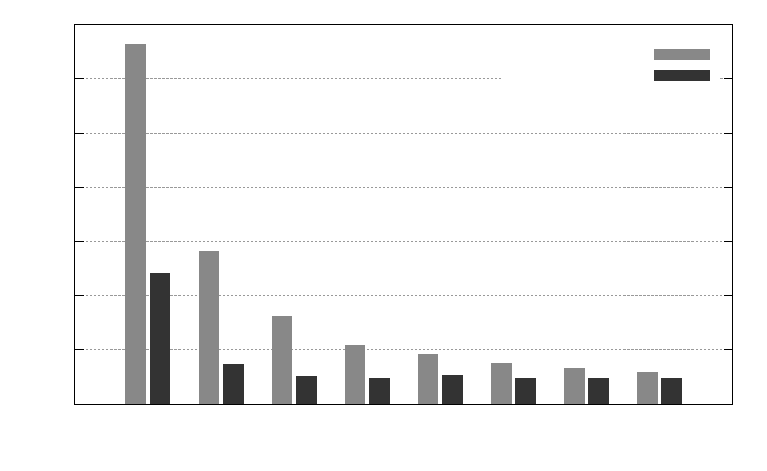
\includegraphics{../data/performance/plots/cores/helios-plot}}%
    \gplfronttext
  \end{picture}%
\endgroup

  \vspace{.5\baselineskip}
  \caption[Einfluss der zur Verfügung stehenden Rechenkerne auf durchschnittliche Laufzeit der Typüberprüfung von Flow und TypeScript]{
    Einfluss der zur Verfügung stehenden Rechenkerne auf durchschnittliche Laufzeit der Typüberprüfung von Flow 0.96 und TypeScript 3.5 der Projekte Components und Helios.
  }

  \vspace{\baselineskip}
  \caption*{
    \small
    Gemessen mit Intel Core i7-6700 CPU mit 3,4~GHz (Prozessor D).
  }

  \label{fig:plot-cores}
\end{figure}

\medbreak
\begingroup
\setlength{\tabcolsep}{7pt}
\begin{table}[tbh]
  \caption[Durchschnittliche Laufzeit in Sekunden, Standardabweichung (s) und relative Veränderung der Zeitspanne (rel. $\Delta$) der vollständigen Typüberprüfung der Projekte Components und Helios durch Flow 0.96 und TypeScript 3.5 bei zunehmender Zahl verfügbarer Rechenkerne~(K).]{Durchschnittliche Laufzeit in Sekunden, Standardabweichung (s) und relative Veränderung der Zeitspanne (rel. $\Delta$) der vollständigen Typüberprüfung der Projekte Components und Helios durch Flow 0.96 und TypeScript 3.5 bei zunehmender Zahl verfügbarer Rechen"=kerne~(K). Gemessen mit Intel Core i7-6700 CPU mit 3,4 GHz (System D).}
  \small
  \begin{tabu} to \textwidth {@{}rrrrrr|rrrrrX@{}}
    \midrule
    {} & \multicolumn{2}{l}{\libertineSB{Flow}} & \multicolumn{2}{l}{\libertineSB{TypeScript}} & {} & \multicolumn{2}{l}{\libertineSB{Flow}} & \multicolumn{2}{l}{\libertineSB{TypeScript}} & {}\\
    \rowfont[c]{} \libertineSB{K} & Laufzeit & s & Laufzeit & s & rel. $\Delta$ & Laufzeit & s & Laufzeit & s & rel. $\Delta$ & {}\\
    \midrule
    1 & 10,59 & 0,03 & 10,13 & 0,03 & -4,3\% & 17,26 & 0,05 & 8,81 & 0,01 & -49,0\% & {} \\
    2 &  6,19 & 0,02 &  6,85 & 0,05 & 10,7\% &  9,61 & 0,04 & 5,44 & 0,04 & -43,4\% & {} \\
    3 &  4,74 & 0,03 &  6,50 & 0,02 & 37,1\% &  7,23 & 0,03 & 5,03 & 0,02 & -30,4\% & {} \\
    4 &  4,05 & 0,03 &  6,43 & 0,02 & 58,8\% &  6,16 & 0,04 & 4,95 & 0,01 & -19,6\% & {} \\
    5 &  3,79 & 0,04 &  6,48 & 0,02 & 71,0\% &  5,82 & 0,03 & 5,04 & 0,15 & -13,4\% & {} \\
    6 &  3,63 & 0,02 &  6,41 & 0,04 & 76,6\% &  5,51 & 0,03 & 4,94 & 0,03 & -10,3\% & {} \\
    7 &  3,52 & 0,02 &  6,40 & 0,03 & 81,8\% &  5,31 & 0,03 & 4,93 & 0,03 &  -7,2\% & {} \\
    8 &  3,42 & 0,02 &  6,40 & 0,03 & 87,1\% &  5,16 & 0,02 & 4,94 & 0,03 &  -4,3\% & {} \\
    \midrule
    {} & \multicolumn{5}{c}{\large\textsc{components}} & \multicolumn{5}{c}{\large\textsc{helios}} & {}\\
    \midrule
  \end{tabu}
  \label{tab:performance-cores}
\end{table}
\endgroup


\subsubsection{Fazit}

Die angestrebte Verbesserung der Performance durch die Migration zu TypeScript kann im vorliegenden Fall nur als teilweise erreicht betrachtet werden, da nur in drei Fällen bei Helios tatsächlich geringere Laufzeiten für eine vollständige Typüberprüfung gemessen wurden. Die stark parallelisierte Architektur von Flow scheint der von TypeScript bezüglich der Geschwindigkeit in den meisten Fällen überlegen. Es wird aber vermutet, dass die Performance von TypeScript deutlich gesteigert werden könnte, wenn auch hier die Berechnung der Typkorrektheit durch mehrere Rechenkerne möglich wäre. Laut Aussage eines leitenden Entwicklers von TypeScript im März 2019 wird die Implementierung von Multithreading im TypeScript Compiler zukünftig in Betracht gezogen~\autocite{TS:MULTICORE}.

\subsection{Zukunftssicherheit und Transparenz der Technologie}

% TODO: artikel: what we've been up to
% TODO: roadmap
% TODO: evtl berechnen wie lang issues im schnitt offen bleiben?
